% **************************************************************************************************************
% A Classic Thesis Style
% An Homage to The Elements of Typographic Style
%
% Copyright (C) 2015 André Miede http://www.miede.de
%
% If you like the style then I would appreciate a postcard. My address
% can be found in the file ClassicThesis.pdf. A collection of the
% postcards I received so far is available online at
% http://postcards.miede.de
%
% License:
% This program is free software; you can redistribute it and/or modify
% it under the terms of the GNU General Public License as published by
% the Free Software Foundation; either version 2 of the License, or
% (at your option) any later version.
%
% This program is distributed in the hope that it will be useful,
% but WITHOUT ANY WARRANTY; without even the implied warranty of
% MERCHANTABILITY or FITNESS FOR A PARTICULAR PURPOSE.  See the
% GNU General Public License for more details.
%
% You should have received a copy of the GNU General Public License
% along with this program; see the file COPYING.  If not, write to
% the Free Software Foundation, Inc., 59 Temple Place - Suite 330,
% Boston, MA 02111-1307, USA.
%
% **************************************************************************************************************
\RequirePackage{fix-cm} % fix some latex issues see: http://texdoc.net/texmf-dist/doc/latex/base/fixltx2e.pdf
\documentclass[ twoside,openright,titlepage,numbers=noenddot,headinclude,%1headlines,% letterpaper a4paper
                footinclude=true,cleardoublepage=empty,abstractoff, % <--- obsolete, remove (todo)
                BCOR=5mm,paper=a4,fontsize=11pt,%11pt,a4paper,%
                american,spanish%
                ]{scrreprt}

%********************************************************************
% Note: Make all your adjustments in here
%*******************************************************
\input{classicthesis-config}

% # Paquetes
\usepackage{amsthm} % para usar \newtheorem y \proof
\usepackage{mathtools} % para usar rcases
\usepackage{enumitem} % pasa usar tag distintos en las enumeraciones
\usepackage{amssymb} % para usar el simbolo de no divide
\usepackage{xeboiboites} % para recuardrar resultados
\usepackage{afterpage} % para añadir paginas en blanco

% # Comandos definidos
\newcommand{\code}{\texttt}
\newcommand\blankpage{%
    \null
    \thispagestyle{empty}%
    \addtocounter{page}{-1}%
    \newpage}
\newcommand{\nuevoteorema}[3] {
    \newbreakabletheorem[small box style={draw=orange!30!black!20,%
    fill=orange!10!black!2,decoration=penciline, decorate, thick},
    big box style={color=orange!30!black!20,fill=orange!30!black!10,thick},
    broken edges={draw=orange!30!black!20,thick,fill=orange!20!black!5,
    decoration={penciline,segment length=.5cm,%
    amplitude=1.3mm},decorate},%
    other edges={decorate,thick}]%
    {#1}{#2}{#3}
}
% ## Comandos para agilizar escritura matemática
\newcommand{\F}{\mathbb{F}}
\newcommand{\Fq}{\mathbb{F}_q}
\newcommand{\Fqca}{\overline{\Fq}}
\newcommand{\Fm}{\mathbb{F}_{2^m}}
\newcommand{\Fp}{\mathbb{F}_p}
\newcommand{\Fpn}{\mathbb{F}_{p^n}}
\renewcommand{\P}{\mathbb{P}}
\newcommand{\A}{\mathbb{A}}
\newcommand{\Kca}{\overline{K}}
\newcommand{\EK}{E(K)}
\newcommand{\EKca}{E(\Kca)}
\newcommand{\EFqca}{E(\Fqca)}
\newcommand{\dega}{\deg(\alpha)}
\DeclareMathOperator{\car}{char}
\newcommand{\phiq}{\phi_q}


% # Estilos de teoremas recuadrados
\theoremstyle{definition} % titulo negrita, cuerpo en recta
\newtheorem{contador}{contador}[chapter]
\nuevoteorema{teorema}{Teorema}{contador}
\nuevoteorema{proposicion}{Proposición}{contador}
\nuevoteorema{lema}{Lema}{contador}
\nuevoteorema{corolario}{Corolario}{contador}
\nuevoteorema{ley de grupo}{Ley de grupo}{contador}
\nuevoteorema{definicion}{Definición}{contador}
% ## Especiales
\nuevoteorema{formulasadiccion}{Fórmulas de adicción}{contador}
\nuevoteorema{teorema2}{Teorema}{}
% # Estilos de teorema no recuadrados
\newtheorem{algoritmo}[contador]{Algoritmo}
\newtheorem{nota}[contador]{Nota}
\newtheorem{ejemplo}[contador]{Ejemplo}
\newtheorem{protocolo}[contador]{Protocolo criptográfico}
% ## Especiales
\newtheorem{metodocuerda}[contador]{Método de la cuerda y la tangente}
\newtheoremstyle{break}% name
  {}%         Space above, empty = `usual value'
  {}%         Space below
  {}% Body font
  {}%         Indent amount (empty = no indent, \parindent = para indent)
  {\bfseries}% Thm head font
  {.}%        Punctuation after thm head
  {\newline}% Space after thm head: \newline = linebreak
  {}%         Thm head spec
\theoremstyle{break}
\newtheorem{algoritmo2}[contador]{Algoritmo}


%********************************************************************
% Bibliographies
%*******************************************************
\addbibresource{Bibliografia.bib}
%\addbibresource[label=ownpubs]{PublicationX.bib}

%********************************************************************
% Hyphenation
%*******************************************************
%\hyphenation{put special hyphenation here}

% ********************************************************************
% GO!GO!GO! MOVE IT!
%*******************************************************
\begin{document}
\frenchspacing
\raggedbottom
\selectlanguage{spanish} % american ngerman
%\renewcommand*{\bibname}{new name}
%\setbibpreamble{}
\pagenumbering{roman}
\pagestyle{plain}
%********************************************************************
% Frontmatter
%*******************************************************
%*******************************************************
% Anteportada
%*******************************************************
\begin{titlepage}
    % if you want the titlepage to be centered, uncomment and fine-tune the line below (KOMA classes environment)
    \begin{addmargin}[-1cm]{-3cm}
    \begin{center}
        \large

        \hfill

        \vfill

        %\includegraphics[width=0.9\textwidth]{Graficos/logo_ugr2}\\[1.4cm]
        \includegraphics[width=4cm]{Graficos/logo_ugr2}

        \vfill

        \spacedallcaps{\mySubtitle} \\ \bigskip

        \spacedlowsmallcaps{\myDegree} \\ \bigskip \bigskip

        \begingroup
            \color{Maroon}\spacedallcaps{\LARGE\myTitle} \\ \bigskip
        \endgroup

        \vfill

        \textbf{Autor} \\
        \myName \\ \medskip

        \textbf{Tutor} \\
        \myProf \\ \medskip

        \vfill

        \spacedlowsmallcaps{\myUni} \\ \medskip

        \myLocation, \myTime %\ -- \myVersion

        \vfill

    \end{center}
  \end{addmargin}
\end{titlepage}

%*******************************************************
% Portada
%*******************************************************
\begin{titlepage}
    % if you want the titlepage to be centered, uncomment and fine-tune the line below (KOMA classes environment)
    \begin{addmargin}[-1cm]{-3cm}
    \begin{center}
        \large

        \hfill

        \vfill

        \begingroup
            \color{Maroon}\spacedallcaps{\LARGE\myTitle} \\ \bigskip
        \endgroup

        \vfill

        \textbf{Autor} \\
        \myName \\ \medskip

        \textbf{Tutor} \\
        \myProf \\ \medskip

    \end{center}
  \end{addmargin}
\end{titlepage}

\cleardoublepage
\cleardoublepage%*******************************************************
% Resumen
%*******************************************************
%\renewcommand{\abstractname}{Abstract}
\pdfbookmark[1]{Resumen}{Resumen}
\begingroup
\let\clearpage\relax
\let\cleardoublepage\relax
\let\cleardoublepage\relax

\chapter*{Resumen}

% Breve resumen del trabajo realizado. Se incluirán seguidamente al menos cinco palabras clave que definan el trabajo a criterio del autor.

En este trabajo se estudia la criptografía asimétrica basada en curvas elípticas, sus protocolos criptográficos y se explica el programa informático desarrollado para trabajar con curvas elípticas y esquemas criptográficos.

Primero se estudian las curvas elípticas sobre un cuerpo arbitrario y se particulariza a cuerpos finitos. Posteriormente, se introduce la criptografía de llave pública con curvas elípticas y se tratan cuestiones de seguridad y de implementación además de ejemplos de esquemas criptográficos. Finalmente, se explica el proceso de diseño, implementación, testeo y documentación del programa informático desarrollado.

\bigskip

\textbf{Palabras clave}: teoría de curvas elípticas, criptografía asimétrica, criptografía con curvas elípticas, cuerpos finitos, protocolos criptográficos.

\endgroup

\vfill

\cleardoublepage\include{PaginasInicialesFinales/ResumenIngles}
\afterpage{\blankpage}
\cleardoublepage%*******************************************************
% Declaration
%*******************************************************
\refstepcounter{dummy}
%\pdfbookmark[0]{Declaration}{declaration}
\pdfbookmark[1]{Declaraciones}{Declaraciones}
\chapter*{}
\thispagestyle{empty}
% TODO: rellenar DNI
Yo, \textbf{\myName}, alumno de la titulación \myDegree de la \textbf{Facultad de Ciencias} y de la \textbf{Escuela Técnica Superior de Ingenierías Informática y de Telecomunicación} de la \textbf{Universidad de Granada}, con DNI XXXXXXXXX, autorizo la ubicación de la siguiente copia de mi Trabajo Fin de Grado en la biblioteca de ambos centros para que pueda ser consultada.
\bigskip

\noindent\textit{\myLocation, \today}

\vspace{3cm}

\begin{flushright}
    \begin{tabular}{m{5cm}}
        \\ \hline
        % TODO: añadir firma
        \centering\myNameShort \\
    \end{tabular}
\end{flushright}

\cleardoublepage%*******************************************************
% Declaration
%*******************************************************
\refstepcounter{dummy}
%\pdfbookmark[0]{Declaration}{declaration}
\chapter*{}
\thispagestyle{empty}
D. \textbf{\myProf}, Profesor del \myDepartment de la Universidad de Granada.

\vspace{0.5cm}

\textbf{Informa:}

\vspace{0.5cm}

Que el presente trabajo, titulado \textit{\textbf{\myTitle}}, ha sido realizado bajo su supervisión por \textbf{\myName}, y autorizo la defensa de dicho trabajo ante el tribunal que corresponda.

\vspace{0.5cm}

Y para que conste, expido y firmo el presente informe en Granada a \underline{\hspace{0.5cm}} de julio de 2016.

\vspace{3cm}

\begin{flushright}
    \begin{tabular}{m{5cm}}
        \\ \hline
        % TODO: añadir firma
        \centering\myProf \\
    \end{tabular}
\end{flushright}

\cleardoublepage%*******************************************************
% Agradecimientos
%*******************************************************
\pdfbookmark[1]{Agradecimientos}{agradecimientos}

\begingroup
\let\clearpage\relax
\let\cleardoublepage\relax
\let\cleardoublepage\relax
\chapter*{Agradecimientos}

Quería agradecer en primer lugar a la Universidad de Granada y sus profesores, por darme la oportunidad de formarme. En especial, al tutor de este trabajo, Pascual Jara, por su ayuda constante a lo largo de este proyecto.

\bigskip

Finalmente, mi mayor agradecimiento a mi familia por no dejar de apoyarme nunca.

\endgroup

\pagestyle{scrheadings}
\cleardoublepage\include{PaginasInicialesFinales/Contenidos}
%********************************************************************
% Mainmatter
%*******************************************************
\cleardoublepage\pagenumbering{arabic}
%\setcounter{page}{90}
% use \cleardoublepage here to avoid problems with pdfbookmark
\cleardoublepage
%\ctparttext{Desarrollo del trabajo matemático-informático.}
%\part{Desarrollo del trabajo}
%\addtocontents{toc}{\protect\clearpage} % <--- just debug stuff, ignore
%**************************
\chapter{Introducción}
\label{ch:Introducción}
%**************************

\subsection{Contextualización}
\label{sub:Contextualización}

% Contextualizar el trabajo explicando antecedentes importantes para el desarrollo realizado y efectuando, en su caso, un estudio de los progresos recientes.

Las curvas elípticas han sido estudiadas por los matemáticos desde la antigüedad y se han utilizado para resolver un abanico variado de problemas. Un ejemplo es el problema de los números congruentes que pregunta por la clasificación de los enteros positivos que aparecen como el aréa de un triangulo rectángulo cuyos lados sean números racionales. Otro ejemplo ha sido el Último Teorema de Fermat que afirma que la ecuación $x^n + y^n = z^n$ no tiene soluciones no triviales para $x, y$ y $z$ cuando $n$ es más grande que 2.

% TODO: a finales de la decada?
La aplicación de las curvas elípticas en la criptografía vino mucho después. En 1985, Neal Koblitz y Victor Miller propusieron independientemente utilizar las curvas elípticas para diseñar sistemas criptográficos de llave pública. Desde entonces, se han publicando una gran cantidad de estudios sobre la seguridad y la eficiencia de las implementaciones de la criptografía con curvas elípticas. A finales de la década de los 90, los sistemas con curvas elípticas empezaron a recibir aceptación comercial cuando organizaciones de estándares acreditadas especificaron protocolos con curvas elípticas y compañías privadas incluyeron dichos protocolos en sus productos de seguridad.

% TODO: debería citaar
Recientemente, se ha comenzado a investigar el uso de curvas hiperelípticas, una generalización de las curvas elíptipcas, para aplicarlas a sistemas criptográficos de llave pública. Sin embargo, estos sistemas son menos seguros o son menos eficientes que los sistemas que usan curvas elípticas.

Uno de los principales problemas al que se enfrenta la criptografía con curvas elípticas, y los principales criptosistemas de llave pública, son los ordenadores cuánticos. En 1994, Shor presentó un algoritmo para un ordenador cuántico capaz de calcular logaritmos discretos y factorizar enteros, principales problemas matemáticos en los que se basa la criptografía de llave pública, de forma eficiente. Sin embargo, hasta la fecha no se ha podido construir un ordenador cuántico con la capacidad suficiente para resolver instancias de estos problemas no triviales.

\subsection{Problema a abordar}
\label{sub:Problema a abordar}

% Describir el problema abordado, de forma que el lector tenga desde este momento una idea clara de la cuestión a resolver o del producto a desarrollar y una visión general de la solución alcanzada.

El problema abordado ha sido la realización de un estudio teórico-práctico sobre las curvas elípticas en criptografía y la implementación de diversos protocolos criptográficos con curvas elípticas.

En el estudio teórico, se abarca la teoría de curvas elípticas desde un punto de vista formal y riguroso. En primer lugar, se tratan las curvas elípticas sobre un cuerpo arbitrario y posteriormente se particulariza a curvas elípticas sobre cuerpos finitos.

%  ya que la literatura sobre este campo es muy extensa.
Nótese que un estudio exhaustivo sobre la teoría de curvas elípticas hubiera sido inviable debido a la enorme extensión que cubre este campo. Serge Lang, autor de esta materia, escribió en la introducción de uno de sus libros: <<It is possible to write endlessly on elliptic curves>>. Por ello, hemos elegido la parte más representativa de esta materia en relación con su aplicación en la criptografía.

En el estudio práctico, se introduce la criptografía de llave pública con curvas elípticas y se hace énfasis en cuestiones de seguridad y de implementación además de explicar algunos ejemplos de esquemas criptográficos con curvas elípticas. Análogamente al estudio teórico, la criptografía con curvas elípticas es un campo muy amplio y de la multitud de aspectos técnicos presentes hemos abarcado los más cruciales.

% TODO: revisar frase (sobre todo el así..)
Por ultimo, se ha desarrollado un programa informático que implementa diversos protocolos criptográficos con curvas elípticas y así aplicar el estudio teórico-práctico realizado. Este programa también permite hacer cálculos con curvas elípticas y cuerpos finitos y ha sido ampliamente testado y bien documentado.

% \subsection{Tecnicas matemáticas e informáticas}
% \label{sub:Tecnicas matemáticas e informáticas}
%
% %  Exponer con claridad las técnicas y áreas matemáticas, así como los conceptos y herramientas de la ingeniería informática que se han empleado.
%
% Matemáticas
% \begin{itemize}
%     \item EC
%     \item Cuerpos finitos
%     \item Geometría algebraica
%     \item Algebra conmutativa
%     \item Teoría de números
%     \item Matemática discreta
% \end{itemize}
%
% Informática
% \begin{itemize}
%     \item Criptografía
%     \item Sistemas de llave pública
%     \item Programación dirigida a objetos
%     \item Cifrado de páginas web
%     \item Complejidad computacional
%     \item Ingeniera del software (doc y testing)
% \end{itemize}

% \subsection{Contenido de la memoria}
% \label{sub:Contenido de la memoria}
%
% % Sintetizar el contenido de la memoria.
%
% \begin{itemize}
%     \item Estudio EC
%     \item Estudio ECC
%     \item Implementacion EC y ECC
%     \item Aplicacion sobre las páginas de la ugr
% \end{itemize}
%
% \subsection{Principales fuentes}
% \label{sub:Principales fuentes}
%
% % Citar las principales fuentes consultadas.
%
% Lawrence.
% Waterloo.
% Menezes.
% Las referencias web.

%**************************
\chapter{Objetivos del trabajo}
\label{ch:Objetivos del trabajo}
%**************************

% En este apartado deberán aparecer con claridad los objetivos inicialmente previstos en la propuesta de TFG y los finalmente alcanzados con indicación de dificultades, cambios y mejoras respecto a la propuesta inicial. Si procede, es conveniente apuntar de manera precisa las interdependencias entre los distintos objetivos y conectarlos con los diferentes apartados de la memoria.

% Se pueden destacar aquí los aspectos formativos previos más utilizados.

Los objetivos inicialmente previstos eran:
\begin{itemize}
    \item Realizar un estudio en profundidad de las curvas elípticas sobre cuerpos finitos y la aritmética de sus puntos.
    \item Implementar algoritmos para trabajar con la aritmética del grupo de una curva elíptica.
    \item Implementar protocolos criptográficos basados en curvas elípticas.
\end{itemize}

Para alcanzar el primer objetivo, estudiamos primero el caso general, esto es, curvas elípticas sobre un cuerpo arbitrario, y depués particularizamos a cuerpos finitos. Como la teoría de curvas elípticas es muy extensa, no hemos podido abarcar todo lo que nos hubiera gustado y hemos tenido que elegir la parte más representativa de esta materia en relación con su aplicación en la criptografía.

Para alcanzar los dos objetivos relacionados con la implementación, previamente realizamos un estudio sobre la criptografía asimétrica con curvas elípticas, haciendo énfasis en los algoritmos y procedimientos que contiene y sus protocolos criptográficos. Análogamente al caso anterior, tuvimos que seleccionar los aspectos más importantes de la criptografía asimétrica con curvas elípticas debido a la multitud de detalles técnicos presentes en este campo.

Con este conocimiento, desarrollamos un programa informático capaz de operar con el grupo de puntos de una curva elíptica y trabajar con protocolos criptográficos.
Para ello también tuvimos que implementar la aritmética modular entre enteros y polinomios y la aritmética de cuerpos finitos. Los protocolos criptográficos implementados y utilizados en aplicaciones reales han tenido en cuenta una multitud de detalles técnicos relacionados con la eficiencia y la seguridad, de los cuales solo los más cruciales han sido tenido en cuenta en nuestra implementación particular.

En la tabla~\ref{tab:Objetivos alcanzandos} mostramos los objetivos finalmente alcanzados y el apartado de la memoria donde se trata cada objetivo.

\begin{table}[p]
  \myfloatalign
  \begin{tabularx}{\textwidth}{Xl} \toprule
    \tableheadline{Objetivo alcanzado} & \tableheadline{Localización}  \\
    \midrule
    Realizar un estudio en profundidad de las curvas elípticas y la aritmética de sus puntos y particularizarlo a curvas elípticas sobre cuerpos finitos. & Capitulo~\ref{ch:Desarrollo matemático} \\
    Realizar un estudio sobre la criptografía asimétrica con curvas elípticas, incluyendo algunos de sus algoritmos y protocolos más importantes. & Sección~\ref{sec:Criptografía con curvas elípticas} \\
    Implementar algoritmos para trabajar con la aritmética modular de enteros y polinomios, de cuerpos finitos y del grupo de una curva elíptica. & Sección~\ref{sec:Criptografía con curvas elípticas con Python} \\
    Implementar protocolos criptográficos basados en curvas elípticas. & Sección~\ref{sec:Criptografía con curvas elípticas con Python} \\
    \bottomrule
  \end{tabularx}
  \caption{Objetivos alcanzandos.}\label{tab:Objetivos alcanzandos}
\end{table}

Por otro lado, la tabla~\ref{tab:Asignaturas más relevantes} muestra las materias del Doble Grado en Matemáticas e Ingeniería Informática más relacionadas con el trabajo.

\begin{table}[p]
  \myfloatalign
  \begin{tabularx}{\textwidth}{X} \toprule
    %\tableheadline{Asignaturas} \\
    %\midrule
    % Matemáticas
    Álgebra I, II, III. \\
    Geometría I, II. \\
    Curvas y superficies. \\
    Álgebra conmutativa computacional. \\
    Teoría de números y criptografía. \\

    % Informática
    Fundamentos de programación. \\
    Metodología de la programación. \\
    Estructura de datos. \\
    Algorítmica. \\
    Fundamentos de ingeniería del software. \\
    Modelos avanzados de computación. \\
    Programación y diseño orientado a objetos. \\
    Seguridad y protección de sistemas informáticos. \\
    \bottomrule
  \end{tabularx}
  \caption{Materias del doble grado relacionadas con el trabajo.}\label{tab:Asignaturas más relevantes}
\end{table}

%**************************
\chapter{Aritmética de las curvas elíptica}
\label{ch:Aritmética de las curvas elíptica}
%**************************

% conceptos han aparecido: extensión de cuerpo, característica

En el apartado~\ref{sec:Introducción} se introducen las curvas elípticas. Se explican las operaciones de grupo adicción y duplicacíon para los puntos de una curva elíptica, junto con su estructura fundamental y otras propiedades.

Las principales referencias usadas en este capítulo han sido~\cite{Washington:2008} y~\cite{Hankerson:2003}.

% TODO: seguir con la introducción de contenidos

\section{Introducción a las curvas elípticas}
\label{sec:Introducción}

% TODO: preguntarle a Pascual por la forma de citar (poner en el encabezado las principales referencias y despues para cosas puntuales usar \cite), pero no en cada definición o resultado no trivial.
\begin{definicion}
\label{def:curva elíptica}
	Una \emph{curva elíptica} $E$ se define por una una ecuación de la forma
	\begin{equation}
	\label{eq:Weierstrass general}
		E : y^2 + a_1 x y + a_3 y = x^3 + a_2 x^2 + a_4 x + a_6
	\end{equation}

	donde $a_1, a_2, a_3, a_4, a_6 \in K$ y $\Delta \neq 0$, donde $\Delta$ es el \emph{discriminante} de $E$ y se define como:

	\begin{align}
		\label{eq:discriminante}
		\begin{rcases}
		\Delta & = -d_2^2 d_8 - 8 d_4^3 - 27 d_6^2 + 9 d_2 d_4 d_6         \\
		d_2    & = a_1^2 + 4 a_ 2                                          \\
		d_4    & = 2 a_4 + 4 a_2                                           \\
		d_6    & = a_3^2 + 4 a_6                                           \\
		d_8    & = a_1^2 a_6 + 4 a_2 a_6 - a_1 a_3 a_4 + a_2 a_3^2 - a_4^2 \\
		\end{rcases}
	\end{align}

	Si $L$ es una extensión del cuerpo $K$, entonces el conjunto de puntos \emph{L-racionales} de $E$ es:
	$$
	E(L) = \{\infty\} \cup \{(x, y) \in L \times L: y^2 + a_1 x y + a_3 y = x^3 + a_2 x^2 + a_4 x + a_6 = 0\}
	$$
\end{definicion}

\begin{nota}[comentarios de la definición~\ref{def:curva elíptica}]\leavevmode
	\begin{itemize}
		\item La ecuación~\eqref{eq:Weierstrass general} se conoce como la \emph{ecuación de Weierstrass}.
		\item Diremos que $E$ \emph{está definida sobre} $K$ y lo notaremos $E/K$. A $K$ lo llamaremos \emph{cuerpo base}.
		\item La condición $\Delta \neq 0$ asegura que la curva elíptica es <<suave>>, esto es, no hay puntos en los que la curva tenga dos o mas rectas tangentes.
		% TODO: rellenar referencia a la forma proyectiva
		% TODO: cambiar si no se hace referencia al proyectivo (página 25 de washington)
		\item El punto $\infty$ es el único punto en la línea del infinito que satisface la forma proyectiva de la ecuación de Weierstrass (véase~\ref{}).
	\end{itemize}
\end{nota}

\begin{ejemplo}[curvas elípticas sobre $\mathbb{R}$]
	Consideramos las curvas elípticas:
	\begin{align*}
		E_1: y^2 & = x^3 - x \\
		E_2: y^2 & = x^3 + x
	\end{align*}
	definidas sobre el cuerpo $\mathbb{R}$ de los números reales. Los puntos $E_1(\mathbb{R})$ y $E_2(\mathbb{R})$ se han representado en la Figura~\ref{fig:curvas elípticas reales}.

	% TODO:hacer la gráfica bien (añadir label, etc, etc)
	\begin{figure}[h]
		\myfloatalign
		\subfloat[$E_1: y^2 = x^3 - x$]
		{\includegraphics[width=.45\linewidth]{gfx/grafo_curva_eliptica_reales_1.pdf}} \quad
		\subfloat[$E_2: y^2 = x^3 + x$]
		{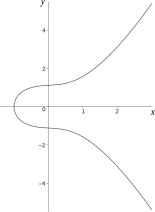
\includegraphics[width=.45\linewidth]{gfx/grafo_curva_eliptica_reales_2.pdf}}
		\caption{Curvas elípticas sobre $\mathbb{R}$}\label{fig:curvas elípticas reales}
	\end{figure}

	% \begin{figure}[h]
	% 	\centering
	% 	\includegraphics[scale=1]{gfx/example_1}
	% 	\caption{Curvas elípticas sobre $\mathbb{R}$}\label{fig:curvas elípticas reales}
	% \end{figure}
\end{ejemplo}

\subsection{Ecuaciones de Weierstrass simplificadas}
\label{sub:Ecuaciones de Weierstrass simplificadas}

\begin{definicion}
	Dos curvas elípticas $E_1$ y $E_2$ definidas sobre $K$ y dadas por las ecuaciones de Weierstrass:
	\begin{align*}
		E_1 &: y^2 + a_1 x y + a_3 y = x^3 + a_2 x^2 + a_4 x + a_6 \\
		E_2 &: y^2 + a_1' x y + a_3' y = x^3 + a_2' x^2 + a_4' x + a_6'
	\end{align*}
	se dicen que son \emph{isomorfas sobre K} si existen $u, r, s, t \in K,\ u \neq 0$, tal que el cambio de variables lineal
	\begin{equation}\label{eq:cambio de variables admisible}
	(x, y) \mapsto (u^2 x + r, u^3 y + u^2 s x + y)
	\end{equation}
	transforma la ecuación $E_1$ en la ecuación $E_2$. La transformación~\eqref{eq:cambio de variables admisible} se llama un cambio de variables admisible.

	El cambio de variables~\eqref{eq:cambio de variables admisible} es el único que deja <<fijo>> el punto del infinito y preserva la forma de la ecuación de Weierstrass. No vamos a entrar en más detalle, pero puede consultar \cite[prop. III.3.1b]{Silverman:2009} para más informácion.
\end{definicion}

% TODO: explicar porqué este cambio de variable referenciando a silverman

Una ecuación de Weierstrass
$$
E:  y^2 + a_1 x y + a_3 y = x^3 + a_2 x^2 + a_4 x + a_6
$$
puede simplificarse considerablemente aplicando cambios de variables admisibles. Usaremos las ecuaciones simplificadas en vez de la general en el resto del trabajo. Vamos a considerar por separado los casos en los que el cuerpo base tenga característica distinta de 2 y 3 o tenga característica 2 o 3.

\begin{enumerate}
	\item Si la característica de $K$ es distinta de $2$ y $3$, entonces el cambio de variables admisible
	$$
	(x, y) \mapsto \left(\frac{x - 3 a_1^2 - 12 a_2}{36}, \frac{y - 3 a_1 x}{216} - \frac{a_1^3 + 4 a_1 a_2 - 12 a_3}{240}\right)
	$$
	transforma $E$ en la curva
	\begin{equation*}\label{eq:ecuación Weierstrass}
		y^2 = x^3 + a x + b
	\end{equation*}
	donde $a, b \in K$. El discriminante de esta curva es $\Delta = -16(4a^3 + 27b^2)$.

	\item Si la característica de K es 2, hay dos casos que considerar. Si $a_1 \neq 0$, entonces el cambio de variables admisible
	$$
	(x, y) \mapsto \left(a_1^2 x + \frac{a_3}{a_1}, a_1^3 y + \frac{a_1^2 a_4 + a_3^2}{a_1^3} \right)
	$$
	transforma $E$ en la curva
	\begin{equation*}
		y^2 + xy = x^3 + a x^2 + b
	\end{equation*}
	% TODO: rellenar referencia
	donde $a, b \in K$. Tales curvas se llaman \emph{no supersingulares} (véase~\ref{}) y tiene discriminante $\Delta = b$. Si $a_1 = 0$, entonces el cambio de variables admisible
	$$
	(x, y) \mapsto (x + a_2, y)
	$$
	transforma $E$ en la curva
	\begin{equation*}
		y^2 + c y = x^3 + a x + b
	\end{equation*}
	% TODO: rellenar referencia
	donde $a, b, c \in K$. Tales curvas se llaman \emph{supersingulares} (véase~\ref{}) y tiene discriminante $\Delta = c^4$.

	\item Si la característica de $K$ es 4, entonces hay dos casos que considerar. Si $a_1^2 \neq -a_2$, entonces el cambio de variables admisible
	$$
	(x, y) \mapsto \left(x + \frac{d_4}{d_2}, y + a_1 x + a_1 \frac{d_4}{d_2} + a_3 \right)
	$$
	donde $d_2 = a_1^2 + a_2$ y $d_4 = a_4 - a_1 a_3$, transforma $E$ en la curva
	\begin{equation*}
		y^2 = x^3 + a x^2 + b
	\end{equation*}
	% TODO: rellenar referencia
	donde $a, b \in K$. Tales curvas se llaman \emph{no supersingulares} (véase~\ref{}) y tiene discriminante $\Delta = -a^3 b$. Si $a_1^2 = -a_2$, entonces el cambio de variables admisible
	$$
	(x, y) \mapsto (x, y + a_1 x + a_3)
	$$
	transforma $E$ en la curva
	\begin{equation*}
		y^2 = x^3 + a x^2 + b
	\end{equation*}
	% TODO: rellenar referencia
	donde $a, b \in K$. Tales curvas se llaman \emph{supersingulares} (véase~\ref{}) y tiene discriminante $\Delta = -a^3$.
\end{enumerate}
\begin{proof}
La demostración completa puede encontrarse en~\cite[sec. III.1]{Silverman:2009}. Se trata simplemente de completar cuadrados y realizar sustituciones, por ello aquí solo mostraremos la demostración de la primera simplifación.

En primer lugar, sumando en la ecuación de Weierstrass~\eqref{eq:Weierstrass general} en ambos lados por $(a_1 a_3 x)/2 + a_3^2/4 + (a_1^2 x^2)/4$, completamos el cuadrado:
$$
\left(y + \frac{a_1 x}{2} + \frac{a_3}{2}\right)^2 = x^3 + \left(a_2 + \frac{a_1^2}{4}\right)x^2 + \left(a_4 + \frac{a_1 a_3}{2}\right)x + \left(a_6 + \frac{a_3^2}{4}\right)
$$
Haciendo $y_1 = y + \frac{a_1 x}{2} + \frac{a_3}{2}$, obtenemos
$$
y_1^2 = x^3 + a_2' x^2 + a_4' x + a_6'
$$
para algunas constantes $a_2', a_4', a_6' \in K$. Finalmente, sustituyendo $x_1 = x + \frac{a_2'}{3}$ resulta
$$
y_1^2 = x_1^3 + a x_1 + b
$$
para algunas constante $a, b \in K$. Para obtener el discriminante $\Delta$ basta sustiuir el valor de las constantes $a_4 = a,\ a_6 = b$ y $a_1 = a_3 = a_2 = 0$ en~\eqref{eq:discriminante}.
\end{proof}

\subsection{Ley de grupo}
\label{sub:Ley de grupo}

Sea $E$ una curva elíptica definida sobre un cuerpo $K$. Hay un \emph{método de la cuerda y la tangente} para sumar dos puntos en $E(K)$ y obtener un tercer punto en $E(K)$. Junto con esta operación aditiva, el conjunto de puntos $E(K)$ forma un gurpo abeliano con $\infty$ como elemento neutro.

La regla aditiva se explica fácilmente geométricamente. Sea $P$ y $Q$ dos puntos distintos de una curva elíptica $E$. Entonces la \emph{suma} $R$, de $P$ y $Q$ esta definido como sigue. Se dibuja una recta $L$ de $P$ a $Q$. Esta recta intersecta la curva elíptica en un tercer punto. Entonces $R$ es la reflexión de este punto sobre el eje-$x$. Esto se puede apreciar en la Figura~\ref{fig:ejemplo adicción}.

El \emph{doble} $R$, de $P$, se define como sigue. Se dibuja la línea tangente $L$ a la curva elíptica en $P$. Esta línea intersecta la curva elíptica en un segundo punto. Entonces $R$ es la reflexión de esto punto sobre el eje-$x$. Esto se puede apreciar en la Figura~\ref{fig:ejemplo duplicación}.

\begin{figure}[h]
  \myfloatalign
  \subfloat[Adicción: $P + Q = R$]{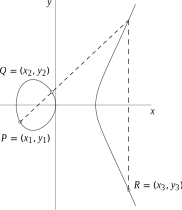
\includegraphics[width=.45\linewidth]{gfx/ejemplo_adiccion.pdf}\label{fig:ejemplo adicción}}
  \quad
  \subfloat[Duplicación: $P + P = P$]{\includegraphics[width=.45\linewidth]{gfx/ejemplo_duplicacion.pdf}\label{fig:ejemplo duplicación}}
  \caption{Adicción y duplicación geométrica de puntos de una curva elíptica}\label{fig:Adicción y duplicación geométrica de puntos de una curva elíptica}
\end{figure}

El hecho de que $L \cap E$, contando multiplicidades, consiste en exactamente tres puntos (no necesariamente distintos) es un caso especial del teorema de Bézout~\cite[sec. I.7.8]{Hartshorne:1977}. Sin embargo, como vamos a dar fórmulas explícitas posteriormente en esta sección, no hay necesidad de usar un teorema general.

%**************************
\chapter{Desarrollo informático}
\label{ch:Desarrollo informático}
%**************************

% TODO: completar introducción
En este capítulo haremos el desarrollo informático sobre criptografía con curvas elípticas. En el apartado~\ref{} hablaremos sobre criptografía asimétrica utilizando curvas elípticas, explicaremos algunos protoclos criptografícos con curvas elípticas en el apartado~\ref{} y por último en el apartado~\ref{} hablaremos del programa desarollado para trabajar con curvas elípticas y protocolos criptográficos.

% TODO: añadir ref si se utilizán más
Las referencias utilizadas para el desarrollo informático han sido sido~\cite{Hankerson:2003}, \cite{Washington:2008} y \cite{Silverman:2009}.

\section{Criptografía con curvas elípticas}
\label{sec:Criptografía con curvas elípticas}
% TODO: hacer introducción

% TODO: poner nota a pie de página mencionando a los descubridores originales del gobierno británico
La criptografía de llave pública (o asimétrica) fue inventada por Diffie y Hellman en 1976, aunque no fueron capaces de encontrar un método práctico para implementar su idea. El primer criptosistema de llave pública llevado a la práctica fue concebido por Rivest, Shamir y Adleman. El criptosistema RSA basa su seguridad en la dificultad de factorizar números grandes. Sin embargo, Diffie y Hellman describieron un algoritmo de intercambio de llaves cuya seguridad se basaba en el logaritmo discreto en $\Fq^*$ y posteriormente ElGamal creó un criptosistema de llave pública basado en el mismo problema. Koblitz y Miller propusieron remplazar el cuerpo finito $\Fq$ con una curva elíptica $E$, con la esperanza de que el logaritmo discreto en el grupo de puntos de una curva elíptca fuera más difícil de resolver que el logaritmo discreto en el grupo multiplicativo de un cuerpo finito. Su intuición conllevó la creación de la criptografía con curvas elípticas.

% TODO: ver si introducir comparación RSA vs ECC o hacer comparación profunda (pag 38 guide, pag 182 wash, pag 388 silver)

En esta sección trataremos el problema del logaritmo discreto y sus ataques y dos aspectos comunes de los protocolos criptográficos que vamos a ver: los parámetros de dominio y las parejas de llaves.

\subsection{Problema del logaritmo discreto}
\label{sub:Problema del logaritmo discreto}

La dificultad del problema del logaritmo discreto es esencial para la seguridad de los criptografía asimétrica sobre curvas elípticas.

\begin{definicion}
    El \emph{problema del logaritmo discreto sobre curvas elípticas (ECDLP)} es: dado una curva elíptica $E$ definida sobre un cuerpo finito $\Fq$, un punto $P \in E(\Fq)$ de orden $n$ y un punto $Q \in \langle P \rangle$, encontrar el entero $k \in [0, n - 1]$ tal que $Q = k P$. El entero $k$ se llama el \emph{logaritmo discreto de $Q$ respecto a la base $P$} y se denota $k = \log_p Q$.
\end{definicion}

El ataque más simple para resolver el ECDLP es el ataque por \emph{fuerza bruta}, esto es, probar todos los valores posibles de $k$ hasta dar con el válido. El tiempo de ejecucción es aproximadamente $n$ pasos en el peor caso y $n / 2$ pasos en el caso medio. Así, el ataque por fuerza bruta puede ser evitado tomando puntos base cuyo orden $n$ suficientemente largo (p. ej. $n > 2^{80}$).

% TODO: mencionar la O grande
El mejor ataque para curvas arbitrarias conocido sobre el ECDLP es la combinación del \emph{algoritmo de Pohlig-Hellman} y del \emph{algoritmo rho de Pollard}, que tiene un complejidad temporal de $O(\sqrt{p})$, esto es, el tiempo de ejecucción es exponencial en $\log{p}$. donde $p$ es el divisor primo más grande de $n$. Para resistir este ataque, se deben elegir puntos base cuyo orden $n$ sea divisible por un primo $p$ suficiente grande (p. ej $p > 2^{160}$).

Además se deben evitar ciertos tipos de curvas para los cuales existen ataques específicos más rápidos que el algoritmo rho de Pollard, llamados \emph{ataques por isomorfismo}. Así pues, se deben evitar curvas \emph{anómalas} (curvas cuyo orden es de la forma $|E(\Fp)| = p$), curvas supersingulares (véase ~\ref{def:supersingular}), curvas con un orden de la forma $|E(\Fq)| = q - 1$ y curvas sobre $\Fm$ si $m$ es compuesto. Adicionalmente habría que comprobar que $n$ no divide a $q^k - 1$ para todo $1 \le k \le C$, donde $C$ es suficientemente grande (si $n > 2^{160}$, entonces $C = 20$ basta).

Puede más información sobre estos ataques en~\cite[cap. 4]{Hankerson:2003} y en~\cite[cap. 4]{Washington:2008}.

\subsection{Parámetros de dominio}
\label{sub:Parámetros de dominio}

Los parámetros de dominio de un esquema criptográfico con curvas elípticas describen una curva elíptica $E$ definida sobre un cuerpo finito $\Fq$, un punto base $P \in E(\Fq)$ y su orden $n$. Los paramétros deben ser elegidos para que el ECDLP sea resistente a los ataques conocidos.

\begin{definicion}
    Los \emph{paramétros de dominio} $D = (q, a, b, P, n)$ están constituidos por:
    \begin{itemize}
        \item El \emph{orden $q$ del cuerpo finito}.
        \item Dos \emph{coeficientes} $a, b \in \Fq$ que definen la ecuación de la curva eliptica $E$ sobre $\Fq$ (p. ej. $y^2 = x^3 + a x + b$ si la característica del cuerpo finito es distinta de 2 y 3 o $y^2 + x y = x^3 + a x^2 + b$ si la característica es 2).
        \item Dos elementos $x_p, y_p \in \Fq$ que definen el punto $P = (x_p, y_p) \in E(\Fq)$ de orden primo. $P$ se conoce como el \emph{punto base}.
        \item El \emph{orden $n$} de $P$.
    \end{itemize}
\end{definicion}

% TODO: ver si cambiar o citar
A la hora de elegir los parámetros de dominio, existen dos opciones. Por un lado, se pueden generar aleatoriamente y posteriormente validarlos para comprobar que describen una curva elíptica segura. Nótese que para cumplir las restricciones de seguridad es necesario determinar el número de puntos de una curva elíptica. Entre los distintos algoritmos para ello (fuerza bruta, el método de multiplicación compleja, \ldots) el mejor es el algoritmo de Schoof-Elkies-Atkin (SEA). En~\cite[cap. 4]{Hankerson:2003} puede encontrar los algoritmos de generación y validación de parámetros de dominio, mientras que en~\cite[cap. XI]{Silverman:2009} puede encontrar un descripción del algoritmo SEA.

Por otro lado, los parámetros de dominio se pueden elegir de algún \emph{estándar}. Organizaciones como el Instituto Nacional de Normas y Tecnología (NIST) o el Grupo de Estándares para la Criptografía Eficiente (SECG), entre muchos otros, publican
parámetros de dominio verificados. En~\cite[apéndice B]{Hankerson:2003} puede encontrar algunas de estas organizaciones y los estándares que han publicado.

\subsection{Pareja de llaves}
\label{sub:Pareja de llaves}

En los protocolos que vamos a ver, cada participante dispondrá de una pareja de llaves, una llave privada (conocida solo por dicho participante) y una llave pública (publicada al resto de participantes). Esta pareja de llaves estará asociada a unos parámetros de dominio particulares. Para generar la pareja de llaves, se elige un punto aleatorio $Q$ en el grupo $\langle P \rangle$. La correspondiente llave privada es $d = \log_p Q$. Si $D = (q, a, b, P, n)$ son los parámetros de dominio, el algoritmo para la generación de llaves es el siguiente:

\begin{algoritmo}\label{alg:pareja de llaves}
    \begin{enumerate}
        \item Seleccionar $d \in [1, n -1]$ aleatoriamente.
        \item Calcular $Q = d P$.
        \item Devolver $(Q, d)$ donde $Q$ es la llave pública y $d$ la llave privada.
    \end{enumerate}
\end{algoritmo}

Nótese que el problema de calcular la llave privada a partir de la llave pública es precisamente el ECDLP. Por eso es crucial que los parámetros de dominio sean seleccionados de tal forma que el ECDLP sea intratable. Además, es necesario que los participantes validen las llave públicas que utilicen ya que existen ataques efectivos si no se hace algunas comprobaciones~\cite[cap. 4]{Hankerson:2003}.

\section{Protocolos criptográficos}
\label{sec:Protocolos criptográficos}

% TODO: intro
Como es común en criptografía, vamos a representar a los participantes que desean comunicarse como Alicia y Bob y representaremos al atacante por Eva.

Este primer protocole que vamos a describir permite a Alicia y Bob intercambiar de forma segura una pieza de información cuyo valor no conoce ninguno de los dos a prori.

\subsection{Protocolo Diffie-Hellman}
\label{sub:Protocolo Diffie-Hellman}

El siguiente procedimiento permite a Alicia y Bob intercambiar de forma segura el valor de un punto en una curva elíptica aunque ninguno de los dos conozca inicialmente el valor del punto.

\begin{protocolo}\label{pc:diffie-hellman}
    \begin{enumerate}
        \item Alicia y Bob concuerdan unos parámetros de dominio $D = (q, a, b, P, n)$.
        \item Alicia calcula su pareja de llaves $(Q_A, d_A)$ según~\ref{alg:pareja de llaves}.
        \item Bob calcula su pareja de llaves $(Q_B, d_B)$ según~\ref{alg:pareja de llaves}.
        \item Alicia y Bob intercambian sus llaves pública $Q_A, Q_B$.
        \item Alicia calcula $d_A Q_B$ y Bob calcula $d_B Q_A$. Ambos cálculos devuelven el punto $d_A d_B P$.
    \end{enumerate}
\end{protocolo}

**************************
\chapter{Conclusiones y vías futuras}
\label{ch:Conclusiones y vías futuras}
%**************************

% Las conclusiones deberán incluir todas aquellas de tipo profesional y académico. Además, se deberá indicar si los objetivos han sido alcanzados totalmente, parcialmente o no alcanzados.
%
% Si hubiese posibles vías claras de desarrollo posterior sería interesante destacarlas aquí, poniéndolas en valor en el contexto inicial del trabajo.
%
% Finalmente vienen las conclusiones y recomendaciones, en las que, a partir de lo planteado en las secciones anteriores, se presentan los resultados del trabajo, según las hipótesis de partida que se exponían en la introducción. Según los casos, aquí se pueden incluir recomendaciones prácticas y futuras líneas de investigación.

Como hemos visto, la teoría de curvas elípticas es una teoría rica, sofisticada y extensa. Sin embargo, uno de sus aspectos más sorprendentes es su aplicación en la criptografía y como supone una mejora de los sistemas criptográficos ampliamente utilizados. Esta aplicación es un muy buen ejemplo de campo interdisciplinar entre las matemáticas y las ciencias de la computación.

Los objetivos propuestos inicialmente se han alcanzando en su totalidad, sin embargo, la criptografía con curvas elípticas abarca mucho más de lo tratado en este trabajo. Existen así numerosas vías de desarrollo posterior, en la que destacamos algunas:
\begin{itemize}
    \item La \emph{criptografía basada en identidad}, cuyos esquemas criptográficos más utilizados se basan en los emparejamientos bilineales de curvas elípticas, como el emparejamiento Weil estudiado en la sección~\ref{subs:Emparejamiento Weil}.
    \item Un estudio más profundo acerca de los ataques sobre el problema del logaritmo discreto con curvas elípticas estudiado en el apartado~\ref{sub:Problema del logaritmo discreto}. Como ya explicamos, la seguridad de los sistemas criptográficos viene determinada por los ataques conocidos y en este trabajo se realizó una mera introducción sobre ellos. Estos ataques presenten ideas muy interesantes y usan resultados sutiles para conseguir la mayor eficiencia.
    \item Las curvas hiperelípticas, una generalización de las curvas elípticas, y su aplicación en la criptografía. Como ya comentamos en la introducción, aún no se han conseguido sistemas basados en curvas hiperelípticas bien más seguros o bien más eficientes que los basados en curvas elípticas. Aún así, es un campo muy reciente y con gran camino por recorrer.
    \item Desarrollo de algoritmos más eficientes. Mucha de la investigación actual sobre criptografía con curvas elípticas se basa en la búsqueda de algoritmos más eficientes para mejorar la velocidad de estos sistemas. Así, se podría hacer un estudio del estado del arte y desarrollar un nuevo algoritmo que suponga un avance en este ámbito.
\end{itemize}

%\include{multiToC} % <--- just debug stuff, ignore for your documents
% ********************************************************************
% Backmatter
%*******************************************************
\appendix
%\renewcommand{\thechapter}{\alph{chapter}}
\cleardoublepage
% TODO: incluir capitulo0A -> apendice
%%********************************************************************
% Apéndice
%*******************************************************
\chapter{Apéndice}
\label{ap:apendice}

% If problems with the headers: get headings in appendix etc. right
%\markboth{\spacedlowsmallcaps{Appendix}}{\spacedlowsmallcaps{Appendix}}

\begin{center}
  \spacedlowsmallcaps{Estudio del envío de credenciales en las páginas web de la Universidad de Granada}
\end{center}

Como aplicación del estudio teórico-práctico realizado en los capítulos \ref{ch:Desarrollo matemático} y \ref{ch:Desarrollo informático}, hemos considerado de interés realizar un estudio sobre el cifrado de las páginas web de la Universidad de Granada. Específicamente, veremos si la transmisión de datos sensibles está cifrada o no.

Antes de presentar este estudio, es necesario introducir brevemente el protocolo \code{HTTPS}.

\section{Introducción a HTTPS}

\code{HTTP} (Hypertext Transfer Protocol) es el protocolo de navegación web más utilizado. Una característica de este protocolo es que envía la información en texto claro, esto es, cualquiera que intercepte el tráfico de red puede leer lo que se está enviando y recibiendo.

Por esta razón, se desarrolló \code{HTTPS} (Hypertext Transfer Protocol Secure), un protocolo de red basado en \code{HTTP} para la transferencia segura de datos. \code{HTTPS} utiliza los protocolos criptográficos \code{SSL/TLS} de la capa de transporte para cifrar el tráfico \code{HTTP}. A nivel más técnico, \code{HTTPS} asegura no solo confidencialidad, sino también autenticación y previene de numerosos ataques como el ataque del hombre en el medio.

\subsection{Ejemplo de ataque sobre HTTP}
\label{sub:Ejemplo de ataque sobre HTTP}

El ejemplo más característico es el siguiente. Supongamos que un usuario conectado a una red wifi abierta accede a una página web mediante \code{HTTP}. Si esta pagina le solicitara al usuario unas credenciales, el usuario las introduciera  y en ese momento un usuario malicioso estuviera analizando los paquetes de la red, el usuario malicioso obtendría fácilmente sus credenciales. De hecho, hoy en día existen programas como \code{Wireshark} \footnote{\url{https://www.incibe.es/CERT/guias_estudios/guias/guia_wireshark}} que hacen del análisis de paquetes una tarea muy sencilla.

La enorme facilidad para llevar a cabo este tipo de ataques y el hecho de que los usuarios no son conscientes de los riesgos \footnote{\url{https://www.osi.es/es/wifi-publica.html}} que supone conectarse a una red wifi abierta, hacen de esta vulnerabilidad un problema serio.

\subsection{Importancia de HTTPS}
\label{sub:Importancia de HTTPS}

Organizaciones internacionales de prestigio como OWASP  \footnote{\url{https://www.owasp.org/index.php/Transport_Layer_Protection_Cheat_Sheet}} o españolas como INCIBE \footnote{\url{https://www.incibe.es/CERT/guias_estudios/guias/guia_sesiones_web}} recomiendan el uso de \code{HTTPS} \emph{como mínimo} en las páginas donde se envíe información sensible.

En un estudio \footnote{\url{https://www.owasp.org/index.php/Top_10_2010-A9-Insufficient_Transport_Layer_Protection}} realizado por OWASP en el año 2010, el noveno riesgo más importante de las aplicaciones web fue la \emph{Protección Insuficiente en la Capa de Transporte}, esto es, cuando el tráfico entre el servidor y el navegador no está protegido debido a la ausencia de cifrado o una mala configuración de los protocolos \code{SSL/TLS}.

Es más, OWASP cataloga como vulnerabilidad \footnote{\url{https://www.owasp.org/index.php/Insecure_Transport}} la ausencia de cifrado en una página web.

Por ello, todos los administradores de sitios web que requieran a los usuarios información sensible, deberían configurar el acceso a dichas páginas mediante \code{HTTPS} sobre \code{SSL/TLS}.

\subsection{Como comprobar si una página utiliza HTTPS}
\label{sub:Como comprobar si una página utiliza HTTPS}

Por desgracia, no todos los sitios web siguen esta medida de seguridad. Por ello, se recomienda que los usuarios sean capaces de reconocer si una página cifra las comunicaciones y en caso negativo, no enviar ningún tipo de dato sensible. La Oficina de Seguridad del Internauta \footnote{\url{https://www.osi.es/es/actualidad/blog/2014/02/28/que-pasa-si-una-pagina-web-no-utiliza-https.html}} ofrece más información al respecto.

En el estudio sobre las páginas web de la Universidad de Granada que hemos realizado, se ha seguido el método descrito por OWASP  \footnote{\url{https://www.owasp.org/images/5/52/OWASP_Testing_Guide_v4.pdf}} para testear el transporte de credenciales. Básicamente, mediante un enfoque de \emph{caja negra} y
el uso del proxy web \code{WebScarab}, se ha simulado la introducción de credenciales y se ha observado las cabeceras de los paquetes para ver si se transmitían mediante \code{HTTP} o \code{HTTPS}.

\section{Estudio de las páginas web de la UGR}

En un primer momento pensábamos que, en atención a las políticas de seguridad y no difusión de datos personales, las páginas de la Universidad de Granada que requerían información sensible estarían protegidas. Sin embargo, hemos comprobado que algunas de ellas no lo están.

Un listado de las páginas visitadas a fecha 30/03/2016 junto con los fallos de seguridad encontrados se presenta a continuación.

\subsection{Primer fallo de seguridad encontrado}

El primer y principal fallo de seguridad que hemos encontrado ha sido la inexistencia de cifrado en el envío de credenciales de las siguientes páginas web:

\begin{itemize}
  \setlength\itemsep{0.1em}
  \item \url{http://fciencias.ugr.es}
  \item \url{http://etsiit.ugr.es}
  \item \url{http://grados.ugr.es/informaticaymatematicas}
  \item \url{http://grados.ugr.es/informatica}
  \item \url{http://grados.ugr.es/matematicas}
  \item \url{http://sucre.ugr.es} (incluyendo \url{http://fciencias.ugr.es/aulas/} y la página de reserva de aulas accesible via \url{http://etsiit.ugr.es})
  \item \url{http://calidad.ugr.es}
  \item \url{http://secretariageneral.ugr.es}
  \item \url{http://archivo.ugr.es}
  \item \url{http://catedras.ugr.es}
  \item \url{http://cicode.ugr.es}
  \item \url{http://editorial.ugr.es}
  \item \url{http://unidadigualdad.ugr.es}
  \item \url{http://biotic.ugr.es/pages/intranet}
  \item \url{http://internacional.ugr.es}
  \item \url{http://ssprl.ugr.es}
\end{itemize}
Suponemos que la lista es mucho más extensa, ya que:
\begin{itemize}
  \item Al igual que \href{http://fciencias.ugr.es}{fciencias.ugr.es} y \href{http://etsiit.ugr.es}{etsiit.ugr.es}, las páginas web de muchos otros centros presentan el mismo fallo.
  \item Al igual que \href{http://grados.ugr.es/informatica}{grados.ugr.es/informatica}, \href{http://grados.ugr.es/matematicas}{grados.ugr.es/matematicas} y \href{http://grados.ugr.es/informaticaymatematicas}{grados.ugr.es/informaticaymatematicas}, las páginas web de muchos otros grados presentan el mismo fallo.
\end{itemize}

Las páginas anteriores disponen de un apartado de \emph{login} y como solo está disponible el protocolo \code{HTTP}  en vez del protocolo \code{HTTPS} , las credenciales podrían ser interceptadas por un usuario malicioso.

Como ya hemos comentado, la solución es deshabilitar \code{HTTP} y utilizar para estas páginas \code{HTTPS}  como método exclusivo de acceso.


\subsection{Segundo fallo de seguridad encontrado}

El segundo fallo de seguridad que hemos encontrado ha sido la coexistencia de envío de credenciales cifradas y no cifradas de las siguientes páginas web:

\begin{itemize}
  \setlength\itemsep{0.1em}
  \item \url{http://oficinavirtual.ugr.es/ai}
  \item \url{http://sede.ugr.es/sede/mis-procedimientos/index.html} (eligiendo sin certificado digital)
\end{itemize}
Las páginas anteriores se pueden acceder tanto con el protocolo \code{HTTP}  como con el protocolo \code{HTTPS}. De este modo, si se acceden mediante \code{HTTP} , presentan la misma vulnerabilidad que el conjunto anterior de páginas web.

La solución es más sencilla. Basta deshabilitar \code{HTTP} y dejar \code{HTTPS}  como el único método de acceso.

Nótese que aunque este listado es más breve contiene una de las páginas más críticas de la UGR, \href{http://oficinavirtual.ugr.es/ai}{oficinavirtual.ugr.es/ai}.

%********************************************************************
% Other Stuff in the Back
%*******************************************************
\cleardoublepage%********************************************************************
% Bibliografía
%*******************************************************

% Se incluirán tanto las fuentes primarias como todas aquellas cuyo peso haya sido menor en la realización del trabajo. Se recomienda un breve comentario de las referencias, ya sea individualizado, por grupos de referencias o global. En caso de incluir URLs de páginas web deberán ir acompañadas de título, autor y fecha de último acceso, entre otros datos relevantes. Se recomienda no abusar de este tipo de fuentes.


% work-around to have small caps also here in the headline
\manualmark
\markboth{\spacedlowsmallcaps{\bibname}}{\spacedlowsmallcaps{\bibname}} % work-around to have small caps also
%\phantomsection
\refstepcounter{dummy}
\addtocontents{toc}{\protect\vspace{\beforebibskip}} % to have the bib a bit from the rest in the toc
\addcontentsline{toc}{chapter}{\tocEntry{\bibname}}
\label{app:bibliography}

\printbibliography

% TODO: escribir comentario de bibliografía

\cleardoublepage

\chapter*{Referencias web}

% TODO: enlazar con el texto

Herramientas utilizadas en el desarrollo del programa informático:

\begin{itemize}
    \item \url{https://www.python.org/}
    \item \url{http://www.sphinx-doc.org/}
    \item \url{http://hypothesis.works/}
    \item \url{https://google.github.io/styleguide/pyguide.html}
\end{itemize}

Recopilación de curvas usadas en criptografía con curvas elípticas:

%\begin{enumerate}[resume]
\begin{itemize}
    \item \url{https://safecurves.cr.yp.to/}
\end{itemize}

% ********************************************************************
% Game Over: Restore, Restart, or Quit?
%*******************************************************
\end{document}
% ********************************************************************
